\begin{figure}[!htbp]
  \centering
  \begin{subfigure}[b]{0.45\textwidth}
    \caption*{Squared Exponential Kernel}
  \end{subfigure}
  \begin{subfigure}[b]{0.45\textwidth}
    \caption*{Exponential Kernel}
  \end{subfigure}

  \begin{subfigure}[b]{0.15\textwidth}
    \caption*{$\Gc^*$}
    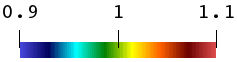
\includegraphics[width=\textwidth]{Chapter4/figures/rainbow_horizontal.png}
  \end{subfigure}
  \begin{subfigure}[b]{0.15\textwidth}
    \caption*{$\psi_c^*$}
    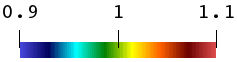
\includegraphics[width=\textwidth]{Chapter4/figures/rainbow_horizontal.png}
  \end{subfigure}
  \begin{subfigure}[b]{0.15\textwidth}
    \caption*{$d$}
    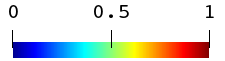
\includegraphics[width=\textwidth]{Chapter4/figures/jet_horizontal.png}
  \end{subfigure}
  \begin{subfigure}[b]{0.15\textwidth}
    \caption*{$\Gc^*$}
    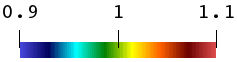
\includegraphics[width=\textwidth]{Chapter4/figures/rainbow_horizontal.png}
  \end{subfigure}
  \begin{subfigure}[b]{0.15\textwidth}
    \caption*{$\psi_c^*$}
    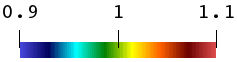
\includegraphics[width=\textwidth]{Chapter4/figures/rainbow_horizontal.png}
  \end{subfigure}
  \begin{subfigure}[b]{0.15\textwidth}
    \caption*{$d$}
    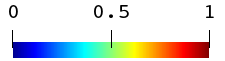
\includegraphics[width=\textwidth]{Chapter4/figures/jet_horizontal.png}
  \end{subfigure}

  \begin{subfigure}[b]{0.15\textwidth}
    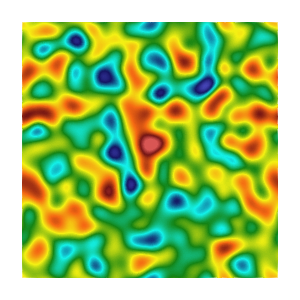
\includegraphics[width=\textwidth]{Chapter4/figures/2D/Gc_sqexp_cartesian_5_5_rho_0_seed_a.png}
    \caption{$L^* = 0.05$}
    \label{fig: Chapter4/2D/Gc_sqexp_cartesian_5_5_rho_0_seed_a}
  \end{subfigure}
  \begin{subfigure}[b]{0.15\textwidth}
    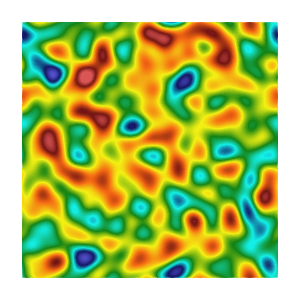
\includegraphics[width=\textwidth]{Chapter4/figures/2D/psic_sqexp_cartesian_5_5_rho_0_seed_a.png}
    \caption{$L^* = 0.05$}
    \label{fig: Chapter4/2D/psic_sqexp_cartesian_5_5_rho_0_seed_a}
  \end{subfigure}
  \begin{subfigure}[b]{0.15\textwidth}
    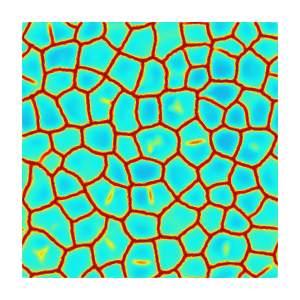
\includegraphics[width=\textwidth]{Chapter4/figures/2D/d_sqexp_cartesian_5_5_rho_0_seed_a.png}
    \caption{}
    \label{fig: Chapter4/2D/d_sqexp_cartesian_5_5_rho_0_seed_a}
  \end{subfigure}
  \begin{subfigure}[b]{0.15\textwidth}
    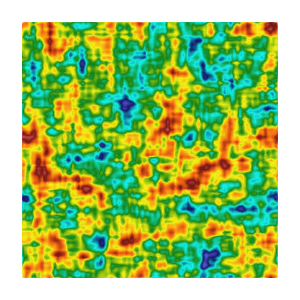
\includegraphics[width=\textwidth]{Chapter4/figures/2D/Gc_exp_cartesian_5_5_rho_0_seed_b.png}
    \caption{$L^* = 0.05$}
    \label{fig: Chapter4/2D/Gc_exp_cartesian_5_5_rho_0_seed_b}
  \end{subfigure}
  \begin{subfigure}[b]{0.15\textwidth}
    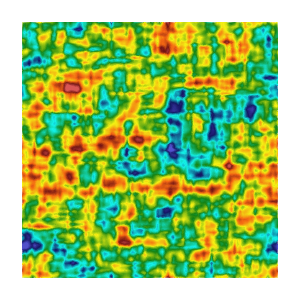
\includegraphics[width=\textwidth]{Chapter4/figures/2D/psic_exp_cartesian_5_5_rho_0_seed_b.png}
    \caption{$L^* = 0.05$}
    \label{fig: Chapter4/2D/psic_exp_cartesian_5_5_rho_0_seed_b}
  \end{subfigure}
  \begin{subfigure}[b]{0.15\textwidth}
    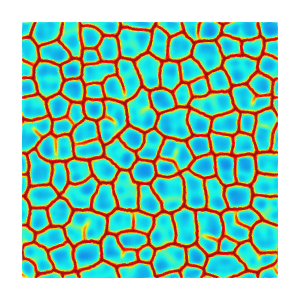
\includegraphics[width=\textwidth]{Chapter4/figures/2D/d_exp_cartesian_5_5_rho_0_seed_b.png}
    \caption{}
    \label{fig: Chapter4/2D/d_exp_cartesian_5_5_rho_0_seed_b}
  \end{subfigure}

  \begin{subfigure}[b]{0.15\textwidth}
    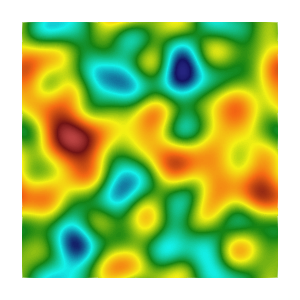
\includegraphics[width=\textwidth]{Chapter4/figures/2D/Gc_sqexp_cartesian_10_10_rho_0_seed_a.png}
    \caption{$L^* = 0.1$}
    \label{fig: Chapter4/2D/Gc_sqexp_cartesian_10_10_rho_0_seed_a}
  \end{subfigure}
  \begin{subfigure}[b]{0.15\textwidth}
    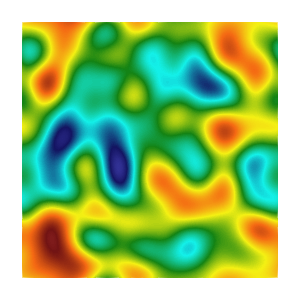
\includegraphics[width=\textwidth]{Chapter4/figures/2D/psic_sqexp_cartesian_10_10_rho_0_seed_a.png}
    \caption{$L^* = 0.1$}
    \label{fig: Chapter4/2D/psic_sqexp_cartesian_10_10_rho_0_seed_a}
  \end{subfigure}
  \begin{subfigure}[b]{0.15\textwidth}
    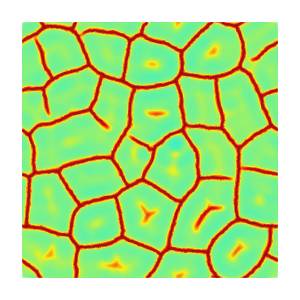
\includegraphics[width=\textwidth]{Chapter4/figures/2D/d_sqexp_cartesian_10_10_rho_0_seed_a.png}
    \caption{}
    \label{fig: Chapter4/2D/d_sqexp_cartesian_10_10_rho_0_seed_a}
  \end{subfigure}
  \begin{subfigure}[b]{0.15\textwidth}
    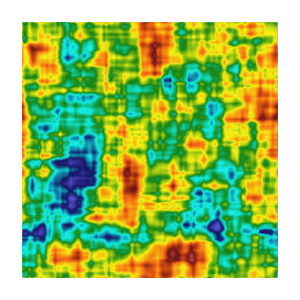
\includegraphics[width=\textwidth]{Chapter4/figures/2D/Gc_exp_cartesian_10_10_rho_0_seed_b.png}
    \caption{$L^* = 0.1$}
    \label{fig: Chapter4/2D/Gc_exp_cartesian_10_10_rho_0_seed_b}
  \end{subfigure}
  \begin{subfigure}[b]{0.15\textwidth}
    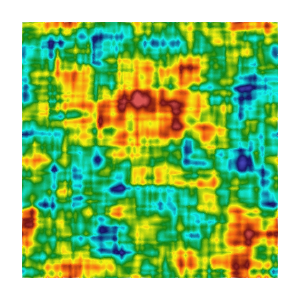
\includegraphics[width=\textwidth]{Chapter4/figures/2D/psic_exp_cartesian_10_10_rho_0_seed_b.png}
    \caption{$L^* = 0.1$}
    \label{fig: Chapter4/2D/psic_exp_cartesian_10_10_rho_0_seed_b}
  \end{subfigure}
  \begin{subfigure}[b]{0.15\textwidth}
    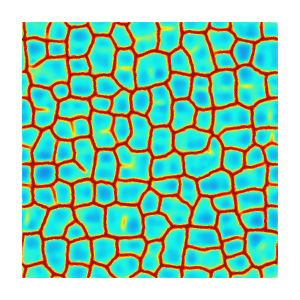
\includegraphics[width=\textwidth]{Chapter4/figures/2D/d_exp_cartesian_10_10_rho_0_seed_b.png}
    \caption{}
    \label{fig: Chapter4/2D/d_exp_cartesian_10_10_rho_0_seed_b}
  \end{subfigure}

  \begin{subfigure}[b]{0.15\textwidth}
    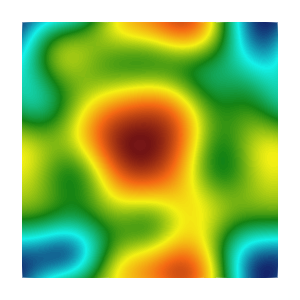
\includegraphics[width=\textwidth]{Chapter4/figures/2D/Gc_sqexp_cartesian_20_20_rho_0_seed_a.png}
    \caption{$L^* = 0.2$}
    \label{fig: Chapter4/2D/Gc_sqexp_cartesian_20_20_rho_0_seed_a}
  \end{subfigure}
  \begin{subfigure}[b]{0.15\textwidth}
    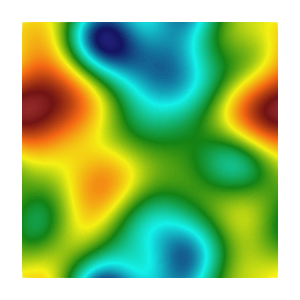
\includegraphics[width=\textwidth]{Chapter4/figures/2D/psic_sqexp_cartesian_20_20_rho_0_seed_a.png}
    \caption{$L^* = 0.2$}
    \label{fig: Chapter4/2D/psic_sqexp_cartesian_20_20_rho_0_seed_a}
  \end{subfigure}
  \begin{subfigure}[b]{0.15\textwidth}
    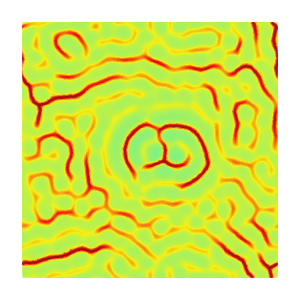
\includegraphics[width=\textwidth]{Chapter4/figures/2D/d_sqexp_cartesian_20_20_rho_0_seed_a.png}
    \caption{}
    \label{fig: Chapter4/2D/d_sqexp_cartesian_20_20_rho_0_seed_a}
  \end{subfigure}
  \begin{subfigure}[b]{0.15\textwidth}
    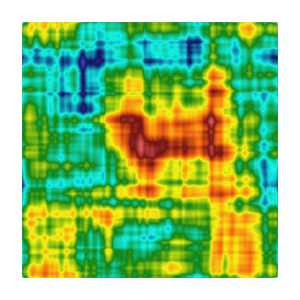
\includegraphics[width=\textwidth]{Chapter4/figures/2D/Gc_exp_cartesian_20_20_rho_0_seed_b.png}
    \caption{$L^* = 0.2$}
    \label{fig: Chapter4/2D/Gc_exp_cartesian_20_20_rho_0_seed_b}
  \end{subfigure}
  \begin{subfigure}[b]{0.15\textwidth}
    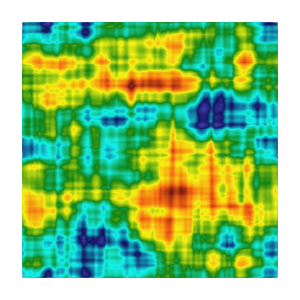
\includegraphics[width=\textwidth]{Chapter4/figures/2D/psic_exp_cartesian_20_20_rho_0_seed_b.png}
    \caption{$L^* = 0.2$}
    \label{fig: Chapter4/2D/psic_exp_cartesian_20_20_rho_0_seed_b}
  \end{subfigure}
  \begin{subfigure}[b]{0.15\textwidth}
    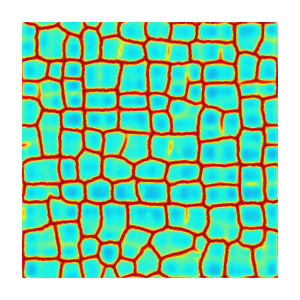
\includegraphics[width=\textwidth]{Chapter4/figures/2D/d_exp_cartesian_20_20_rho_0_seed_b.png}
    \caption{}
    \label{fig: Chapter4/2D/d_exp_cartesian_20_20_rho_0_seed_b}
  \end{subfigure}
  \caption{Damage fields resulting from six pairs of realizations with different correlation models and normalized correlation lengths. The left three pairs (a-b, g-h, m-n) are realizations obtained with a PSE covariance function, while the right three pairs (d-e, j-k, p-q) are samples generated with a PE covariance function. Energy release rate $\Gc$ and the critical fracture energy $\psi_c$ have a coefficient of variation of $0.03$, and normalized spatial correlation length $L^*$ of (a-b, d-e) $0.05$ (g-h, j-k) $0.1$ (m-n, p-q) $0.2$ The corresponding damage fields are shown in (c, f, i, l, o, r), respectively. In these results, independent realizations of the underlying Gaussian fields are used.}
  \label{fig: Chapter4/2D/compare_correlation_length}
\end{figure}
